% REMEMBER: You must not plagiarise anything in your report. Be extremely careful.

\documentclass{l4proj}

    
%
% put any additional packages here
%

\begin{document}

%==============================================================================
%% METADATA
\title{Level 4 Project - Virtual Turing Tumble}
\author{Luke Gall, 2298070g}
\date{September 14, 2018}

\maketitle

%==============================================================================
%% ABSTRACT
\begin{abstract}
    Every abstract follows a similar pattern. Motivate; set aims; describe work; explain results.
    \vskip 0.5em
    ``XYZ is bad. This project investigated ABC to determine if it was better. 
    ABC used XXX and YYY to implement ZZZ. This is particularly interesting as XXX and YYY have
    never been used together. It was found that  
    ABC was 20\% better than XYZ, though it caused rabies in half of subjects.''
\end{abstract}

%==============================================================================

% EDUCATION REUSE CONSENT FORM
% If you consent to your project being shown to future students for educational purposes
% then insert your name and the date below to  sign the education use form that appears in the front of the document. 
% You must explicitly give consent if you wish to do so.
% If you sign, your project may be included in the Hall of Fame if it scores particularly highly.
%
% Please note that you are under no obligation to sign 
% this declaration, but doing so would help future students.
%
\def\consentname {Luke Gall} % your full name
\def\consentdate {20 March 2020} % the date you agree
%
\educationalconsent


%==============================================================================
\tableofcontents

%==============================================================================
%% Notes on formatting
%==============================================================================
% The first page, abstract and table of contents are numbered using Roman numerals and are not
% included in the page count. 
%
% From now on pages are numbered
% using Arabic numerals. Therefore, immediately after the first call to \chapter we need the call
% \pagenumbering{arabic} and this should be called once only in the document. 
%
% Do not alter the bibliography style.
%
% The first Chapter should then be on page 1. You are allowed 40 pages for a 40 credit project and 30 pages for a 
% 20 credit report. This includes everything numbered in Arabic numerals (excluding front matter) up
% to but excluding the appendices and bibliography.
%
% You must not alter text size (it is currently 10pt) or alter margins or spacing.
%
%
%==================================================================================================================================
%
% IMPORTANT
% The chapter headings here are **suggestions**. You don't have to follow this model if
% it doesn't fit your project. Every project should have an introduction and conclusion,
% however. 
%
%==================================================================================================================================
\chapter{Introduction}

% reset page numbering. Don't remove this!
\pagenumbering{arabic} 


Why should the reader care about what are you doing and what are you actually doing?
\section{Guidance}

\textbf{Motivate} first, then state the general problem clearly. 

\section{Writing guidance}
\subsection{Who is the reader?}

This is the key question for any writing. Your reader:

\begin{itemize}
    \item
    is a trained computer scientist: \emph{don't explain basics}.
    \item
    has limited time: \emph{keep on topic}.
    \item
    has no idea why anyone would want to do this: \emph{motivate clearly}
    \item
    might not know \emph{anything} about your project in particular:
    \emph{explain your project}.
    \item
    but might know precise details and check them: \emph{be precise and
    strive for accuracy.}
    \item
    doesn't know or care about you: \emph{personal discussions are
    irrelevant}.
\end{itemize}

Remember, you will be marked by your supervisor and one or more members
of staff. You might also have your project read by a prize-awarding
committee or possibly a future employer. Bear that in mind.

\subsection{References and style guides}
There are many style guides on good English writing. You don't need to
read these, but they will improve how you write.

\begin{itemize}
    \item
    \emph{How to write a great research paper} \cite{Pey17} (\textbf{recommended}, even though you aren't writing a research paper)
    \item
    \emph{How to Write with Style} \cite{Von80}. Short and easy to read. Available online.
    \item
    \emph{Style: The Basics of Clarity and Grace} \cite{Wil09} A very popular modern English style guide.
    \item
    \emph{Politics and the English Language} \cite{Orw68}  A famous essay on effective, clear writing in English.
    \item
    \emph{The Elements of Style} \cite{StrWhi07} Outdated, and American, but a classic.
    \item
    \emph{The Sense of Style} \cite{Pin15} Excellent, though quite in-depth.
\end{itemize}

\subsubsection{Citation styles}

\begin{itemize}
\item If you are referring to a reference as a noun, then cite it as: ``\citet{Orw68} discusses the role of language in political thought.''
\item If you are referring implicitly to references, use: ``There are many good books on writing \citep{Orw68, Wil09, Pin15}.''
\end{itemize}

There is a complete guide on good citation practice by Peter Coxhead available here: \url{http://www.cs.bham.ac.uk/~pxc/refs/index.html}. 
If you are unsure about how to cite online sources, please see this guide: \url{https://student.unsw.edu.au/how-do-i-cite-electronic-sources}.

\subsection{Plagiarism warning}

\begin{highlight_title}{WARNING}
    
    If you include material from other sources without full and correct attribution, you are commiting plagiarism. The penalties for plagiarism are severe.
    Quote any included text and cite it correctly. Cite all images, figures, etc. clearly in the caption of the figure.
\end{highlight_title}


%==================================================================================================================================
\chapter{Background}
What did other people do, and how is it relevant to what you want to do?
\section{Guidance}
\begin{itemize}    
    \item
      Don't give a laundry list of references.
    \item
      Tie everything you say to your problem.
    \item
      Present an argument.
    \item Think critically; weigh up the contribution of the background and put it in context.    
    \item
      \textbf{Don't write a tutorial}; provide background and cite
      references for further information.
\end{itemize}


If I wanted this to focus more for school children. I could try and either target high school or primary and if so maybe talk to the teachers there?

Each puzzle in the starting book has a start set up and a list of available parts they could use, solutions are also given, so puzzles and the right output could be tracked in an app?


% This is where I should put any notes when researching the turing tumble or any virtual comterparts
Turing Tumble is a marble game that can build mechanical computers using various components and gears
Can help teach people how simple switches work which act as the building block to computers. Can teach logic gates, truth tables, conditionals, binary etc

The online version they recommended is very much just the game, could look at making it more of an edu tool by having the puzzles available online and maybe making my own?
Depends if I want it to be used in class rooms for school children in schools where they won't want to get the physical boards due to practice

The balls act as the electricity going through the board

The game board has two flippers, one that releases the blue ball and one that releases the red ones
6 different parts
Ramp directs balls left or right depending on which way it is put in, this moves a ball along the vertical track. These are like wires in normal computing terms
Crossover lets ball paths cross over, so can cross paths that some balls may have. Crossover acts as 2 wires crossing over each other, but not touching
bit, points left or right storing logic. These act as switches which allow the balls to change the course of the next set of electricity 

Interceptor stops any more balls being released, if the ball stops, 'electricity' stops meaning it no longer runs
Gears and gear bits are the components that help make the board turing complete, the bit part stores logic 

Gears and gear bits let other gear bits to turn each other. Can turn gear bits above, side or below them. Needs to be used in combination with gears as they aren't weighted correctly overwise
By using gears we can send info back up the board, so we could send up to the top that a register is above a certain number i.e. for loops
Different combinations of gear bits and bits made different logical pieces, like the latch which lets one blue left and the rest right (2 gear bits top left and bottom with a gear)
Set switch lets you make all bits point in a certain direction, lets you test the direction (bit value) without changing it
Can make a flip flop using gear and gear bits to remember info about it before it drops

This switch can be used to check overflow etc. The combinations that gears and gear bit could be made to do could be explored?


Features that can be improved upon with virtual one online, no save Elements, no login etc. Could be useful? Could encourage people to make puzzles online? 
\emph{Notes on Java Swing}
For java swing, intellij has a swing Ui designer which can be used to automatically add different components to the app without needing to code from scratch
Has a main JFrame which will seems to act as the main desktop app panel that buttons, etc can be placed in. 
Hovering over the components in Intellj doesn't give too much information into what they actually do are why we need them. Could be someone to focus on improving.

The Java swing API has it's main super class as a Component (Object is above this like every java class). It can then be a Container or JComponent. Where a container is either a window or a panel, and the 
components are labels, lists, tables etc. 

Swing isn't really designed for animations, java fx is recommended instead


\emph{Angular vs React} 
Angular is made and maintained by Google using the Typescript as it's main language

React is a front end JS lib for building UI interfaces, made by facebook. More interaction based way of working with the UI Elements

React uses a virtual DOM so would be quicker to re-write elements of HTML Doc (Could include the board pieces)
Angular uses a real DOM so it needs to update the entire HTML tree even for little changes

React is smaller and therefore faster to load up

I already have a bit of knowledge of angular so it might be easier to start with

matter js could be used, plus also animejs and angular has it's own animation library

\emph{React notes}
These notes were taken while undertaking the official react tutorial

Mainly about composing complex UIs from lots of components which are smaller and more singular pieces of code
React will re update and render the components if the data changes.

Reach component class takes in prop and returns a react Element
Can put any JS expressions inside the JSX, so could be a different react class (say a component for the turing tumble)

Parent components can pass data down to child Elements using props, don't think it can go the other way 
Components have state. State can be considered private 

Children props can pass state to each other using shared state stored in the parent component. Parent component can pass the state back down to the children by using props
Keeps the child components in sync

In the tutorial we push state up from the lower down child component so it gets state from it's parent and uses the function provided by it. Making it a controlled component
The tutorial recommends always keeping state immutable and replacing this with new objects instead of changing the existing state for error handling and the ability to check changes more easily in the future
Helps the react engine know when it should update it's rendering 

\emph{Angular vs React vs Vue} 
Frameworks don't equal library's. Libs are pre written code with classes, functions etc, can download these from npm or github
Frameworks include a large stack of functions and help the dev use the various features that would otherwise need to be made before the real site can be done, i.e. routing etc

React is only the UI library would need other technologies to handle any backend (if needed) for example
Vue can let you use JS or Typescipt, but Angular's documentation is all in Typescript but can use normal JS or Dart if needed. 
This makes it good for devs form OO background tho. Angular forces the three file approach to a component while react and vue don't
React is one way binding only which may be an issue. 

\emph{Angular notes} 

I know a little bit of angular already so it wouldn't be a complete deep dive into web dev and could probably help save some hours.
It is fully component based, the components are the main building tools for the framework, each component consists of Typescript, html and css files 
Components are organised hierarchy, this will help force a good layout for my code and will help encourage good practices 
Can support data flow from component to the template - property
    template to the component - event
Can two way bind using these, using a fairly complex background of watchers
Got a slightly steeper learning curve by all accounts 
Typescript is pretty similar to Java or C

\emph{p5}

p5 could be used as a drawing library but I would need to spend some more time looking at it

\emph{Matter js notes (https://brm.io/matter-js/)}
It is a 2D physics engine for shapes and objects, that could be useful to model the marbles going down the slope of the game board
Matter js has an internal engine that updates the animations for us

engine has a timescale object which will slow down animations, which could be useful
x, y starts from top left.
This is a very powerful library with some very interesting examples on their site, this could be a very powerful tool to use to make the envo but it may be difficult to apply the logic of the balls and components, may be easier to 
focus on the logic then add some animation?

Engine is the module for creating and maintains the physics engine while render is the module that visualizes the objects moving
World module is used to provide methods and props to create and manipulate the world, i.e. gravity
Bodies is circles rectangles and other common solid Bodies
body is used to manipulate properties of bodies ie density, velocity etc
Composites allow a quick creation of multiple bodies like a stack of rectangles 

It would definitely be possible to create turing tumble using this library it might just be too powerful for what we need 

% SHOULD MAYBE LOOK AT WCAG
\emph{Online board games}
Tabletop simulator is the most popular game that allows people to play board games in a 3d desktop game that allows multiple people to play 'physical' like online board games.
The player can touch, pick up and move objects which can interact with the board game. Can be a bit complicated for new users however and is very reliant on learning the controls and 
playing the game 'physically'. There is a large mod scene for this game which allows new games and versions to be added by fans of the game creating a large ecosystem of different games for people to play.
The rules for board games need to enforced by the players, it is more a sandbox for the game pieces to exist in which users will manipulate them like in real life to follow the play of the game.
This is the more 'hardcore' version for people serious about playing 3d versions of board games with great community made games and lots of mod-ability.

This game is on the game platform Steam, it also contains a lot of separate virtual versions of popular board games that can be purchased separately which have various levels of polish and online aspects.
Including a GoT board game or versions of Monopoly.

In terms of browser based online board games there is Boardgame Arena which is free online but offers paid exclusive content including better UI or more popular
games. Only the host is required to have the premium games that allows friends to play them together with other people that have the free version. Unlike tabletop simulator
the rules are enforced and it includes tooltips to ensure people can understand the rules as they play the game. It has a fairly simple look and feel to the board games
by using only a top down 2d view on the board. Which makes it easier on slower computers but doesn't make it the most visually appealing. 
Focusing more on logic instead of look and feel while keeping the game 2d will make it more accessible to a wider audience while reducing load on slower PCs.

Many educational games exist online aimed at providing a family friendly and fun way for kids to learn and have fun. Some are made by large charities including Animal Jam made by NatGeo. 
Tinybob has a wide variety of online games aimed at teaching children different subjects. The visuals are very applying and there is a great sense of style and attention put into the games, leading to many awards for the company 
and it's various games. Including ones learning the body, simple physics, the Earth and some Mammals. If I was to go down a more kid focused educational route
these games would be ones to look at.

%==================================================================================================================================
\chapter{Analysis/Requirements}
What is the problem that you want to solve, and how did you arrive at it?

% Write up of Turing Tumble Pieces

\emph{Ramp} 
The Ramp component is the simplest component and acts as a 'wire' in the computer metaphor that persists throughout the components. 
The Ramp sends a ball either right or left depending on the direction the curved end is facing, the ramp doesn't care which way the ball enters
the component, it will send right / left for a ball entering from the top right or left of the component. This piece is reversible in order to change the direction
it faces. As the balls aren't allowed to drop freely until they reach the end, the ramp is the most common way to direct the balls to the desired location.
This components representation in code should store the direction it is facing which will be the direction it sends the ball or 'electricity' down.

\emph{Crossover}
The Crossover is a non reversible piece that continues the direction a ball is travelling into the component but allows the balls to enter from either side.
If a ball enters from the top left, travelling to the bottom right, it will leave the bottom right side of the crossover continuing it's direction. As this is a 
static piece, the crossover can't be reversed and will always act the same way. This piece is metaphorically equivalent to wires crossing over in chips, it allows paths created 
using ramps and other components to cross over each other.

\emph{Bit}
The Bit component acts as a metaphorical switch that will change the direction the next ball will travel based on if it is on (pointing to the right) or off (pointing to the left).
If the bit is pointing to the right (on) send the balls to the left no matter which direction they enter from. Send the balls to the right if the switch is pointing to the left (off).
However when a ball passes through a bit it changes the direction it is facing so it isn't a perfect analogy when comparing them to switches inside circuits. These components can be used to represent registers
that store bit values which can then be used to represent values in binary representation.
This component will need to store the direction it's facing as it's only main property.

\emph{Interceptor}
This component catches a ball and stops the execution of the turing tumble as the marble will no longer be able to reach the end of the board and release another marble. 
By using the metaphor of electricity this component stops the electricity from flowing through the computer meaning it will stop execution.
This component is similar to a shutoff switch inside a regular computer. It will not store any properties but should be able to change the position of the ball to static and 
stop the run time of the board.

\emph{Gear}
Gears are the only components that can be placed on pegs instead of slots on the board and act as connections between a number of gear bits. They turn either 90 left or right. They will need a turn function.

\emph{Gear Bit}
This component is a like a bit in that it stores state by pointing left or right and will send a ball in the opposite direction it is facing and then change direction.
A Gear Bit not connected to a Gear will act and behave exactly like a normal Bit component. When a gear bit changes direction it will also turn any connecting gears this direction which can 
then in turn change other gears and gear bits. The combination of this component and the gear makes the game Turing Complete. 
Information can only be sent down the board unless using these components which can then be used to affect components above the gear bit that gets switched.
This component like the bit will need to be able to store it's direction (state) and then turn itself and any connecting gears.

Using a combination of gear and gear bits we can make new logical components like latches, fixed position switches, set switches and flip flops. The logic of these
new composite components could be explored plus the creation of new components that provide different logic.
\section{Guidance}
Make it clear how you derived the constrained form of your problem via a clear and logical process. 

%==================================================================================================================================
\chapter{Design}
How is this problem to be approached, without reference to specific implementation details? 
\section{Guidance}
Design should cover the abstract design in such a way that someone else might be able to do what you did, but with a different language or library or tool.

%==================================================================================================================================
\chapter{Implementation}
What did you do to implement this idea, and what technical achievements did you make?
\section{Guidance}
You can't talk about everything. Cover the high level first, then cover important, relevant or impressive details.



\section{General points}

These points apply to the whole dissertation, not just this chapter.



\subsection{Figures}
\emph{Always} refer to figures included, like Figure \ref{fig:relu}, in the body of the text. Include full, explanatory captions and make sure the figures look good on the page.
You may include multiple figures in one float, as in Figure \ref{fig:synthetic}, using \texttt{subcaption}, which is enabled in the template.



% Figures are important. Use them well.
\begin{figure}
    \centering
    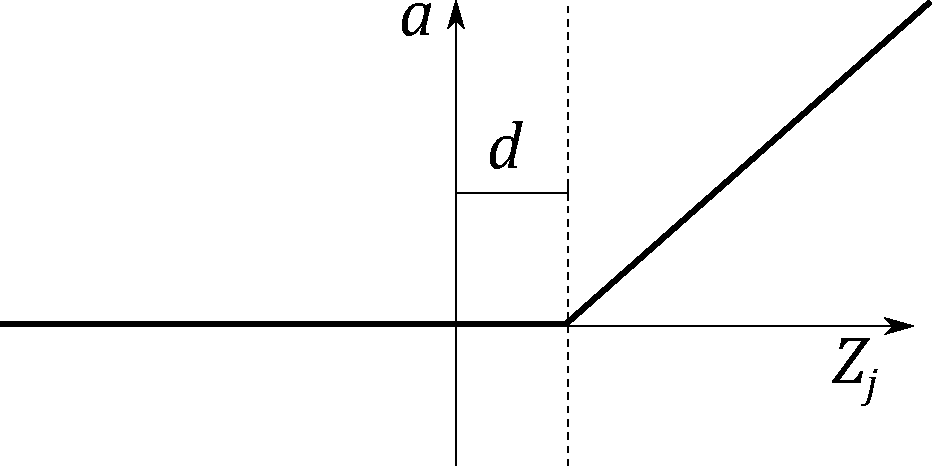
\includegraphics[width=0.5\linewidth]{images/relu.pdf}    

    \caption{In figure captions, explain what the reader is looking at: ``A schematic of the rectifying linear unit, where $a$ is the output amplitude,
    $d$ is a configurable dead-zone, and $Z_j$ is the input signal'', as well as why the reader is looking at this: 
    ``It is notable that there is no activation \emph{at all} below 0, which explains our initial results.'' 
    \textbf{Use vector image formats (.pdf) where possible}. Size figures appropriately, and do not make them over-large or too small to read.
    }

    % use the notation fig:name to cross reference a figure
    \label{fig:relu} 
\end{figure}


\begin{figure}
    \centering
    \begin{subfigure}[b]{0.45\textwidth}
        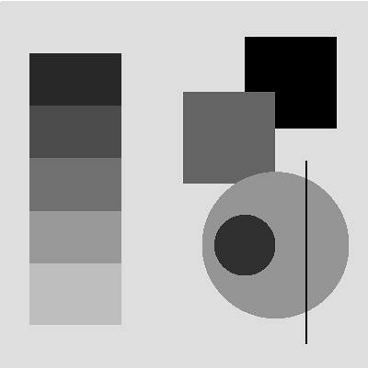
\includegraphics[width=\textwidth]{images/synthetic.png}
        \caption{Synthetic image, black on white.}
        \label{fig:syn1}
    \end{subfigure}
    ~ %add desired spacing between images, e. g. ~, \quad, \qquad, \hfill etc. 
      %(or a blank line to force the subfigure onto a new line)
    \begin{subfigure}[b]{0.45\textwidth}
        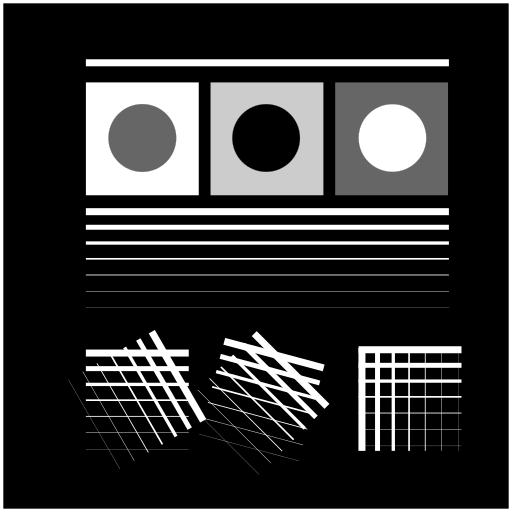
\includegraphics[width=\textwidth]{images/synthetic_2.png}
        \caption{Synthetic image, white on black.}
        \label{fig:syn2}
    \end{subfigure}
    ~ %add desired spacing between images, e. g. ~, \quad, \qquad, \hfill etc. 
    %(or a blank line to force the subfigure onto a new line)    
    \caption{Synthetic test images for edge detection algorithms. \subref{fig:syn1} shows various gray levels that require an adaptive algorithm. \subref{fig:syn2}
    shows more challenging edge detection tests that have crossing lines. Fusing these into full segments typically requires algorithms like the Hough transform.
    This is an example of using subfigures, with \texttt{subref}s in the caption.
    }\label{fig:synthetic}
\end{figure}

\clearpage

\subsection{Equations}

Equations should be typeset correctly and precisely. Make sure you get parenthesis sizing correct, and punctuate equations correctly 
(the comma is important and goes \textit{inside} the equation block). Explain any symbols used clearly if not defined earlier. 

For example, we might define:
\begin{equation}
    \hat{f}(\xi) = \frac{1}{2}\left[ \int_{-\infty}^{\infty} f(x) e^{2\pi i x \xi} \right],
\end{equation}    
where $\hat{f}(\xi)$ is the Fourier transform of the time domain signal $f(x)$.

\subsection{Algorithms}
Algorithms can be set using \texttt{algorithm2e}, as in Algorithm \ref{alg:metropolis}.

% NOTE: line ends are denoted by \; in algorithm2e
\begin{algorithm}
    \DontPrintSemicolon
    \KwData{$f_X(x)$, a probability density function returing the density at $x$.\; $\sigma$ a standard deviation specifying the spread of the proposal distribution.\;
    $x_0$, an initial starting condition.}
    \KwResult{$s=[x_1, x_2, \dots, x_n]$, $n$ samples approximately drawn from a distribution with PDF $f_X(x)$.}
    \Begin{
        $s \longleftarrow []$\;
        $p \longleftarrow f_X(x)$\;
        $i \longleftarrow 0$\;
        \While{$i < n$}
        {
            $x^\prime \longleftarrow \mathcal{N}(x, \sigma^2)$\;
            $p^\prime \longleftarrow f_X(x^\prime)$\;
            $a \longleftarrow \frac{p^\prime}{p}$\;
            $r \longleftarrow U(0,1)$\;
            \If{$r<a$}
            {
                $x \longleftarrow x^\prime$\;
                $p \longleftarrow f_X(x)$\;
                $i \longleftarrow i+1$\;
                append $x$ to $s$\;
            }
        }
    }
    
\caption{The Metropolis-Hastings MCMC algorithm for drawing samples from arbitrary probability distributions, 
specialised for normal proposal distributions $q(x^\prime|x) = \mathcal{N}(x, \sigma^2)$. The symmetry of the normal distribution means the acceptance rule takes the simplified form.}\label{alg:metropolis}
\end{algorithm}

\subsection{Tables}

If you need to include tables, like Table \ref{tab:operators}, use a tool like https://www.tablesgenerator.com/ to generate the table as it is
extremely tedious otherwise. 

\begin{table}[]
    \caption{The standard table of operators in Python, along with their functional equivalents from the \texttt{operator} package. Note that table
    captions go above the table, not below. Do not add additional rules/lines to tables. }\label{tab:operators}
    %\tt 
    \rowcolors{2}{}{gray!3}
    \begin{tabular}{@{}lll@{}}
    %\toprule
    \textbf{Operation}    & \textbf{Syntax}                & \textbf{Function}                            \\ %\midrule % optional rule for header
    Addition              & \texttt{a + b}                          & \texttt{add(a, b)}                                    \\
    Concatenation         & \texttt{seq1 + seq2}                    & \texttt{concat(seq1, seq2)}                           \\
    Containment Test      & \texttt{obj in seq}                     & \texttt{contains(seq, obj)}                           \\
    Division              & \texttt{a / b}                          & \texttt{div(a, b) }  \\
    Division              & \texttt{a / b}                          & \texttt{truediv(a, b) } \\
    Division              & \texttt{a // b}                         & \texttt{floordiv(a, b)}                               \\
    Bitwise And           & \texttt{a \& b}                         & \texttt{and\_(a, b)}                                  \\
    Bitwise Exclusive Or  & \texttt{a \textasciicircum b}           & \texttt{xor(a, b)}                                    \\
    Bitwise Inversion     & \texttt{$\sim$a}                        & \texttt{invert(a)}                                    \\
    Bitwise Or            & \texttt{a | b}                          & \texttt{or\_(a, b)}                                   \\
    Exponentiation        & \texttt{a ** b}                         & \texttt{pow(a, b)}                                    \\
    Identity              & \texttt{a is b}                         & \texttt{is\_(a, b)}                                   \\
    Identity              & \texttt{a is not b}                     & \texttt{is\_not(a, b)}                                \\
    Indexed Assignment    & \texttt{obj{[}k{]} = v}                 & \texttt{setitem(obj, k, v)}                           \\
    Indexed Deletion      & \texttt{del obj{[}k{]}}                 & \texttt{delitem(obj, k)}                              \\
    Indexing              & \texttt{obj{[}k{]}}                     & \texttt{getitem(obj, k)}                              \\
    Left Shift            & \texttt{a \textless{}\textless b}       & \texttt{lshift(a, b)}                                 \\
    Modulo                & \texttt{a \% b}                         & \texttt{mod(a, b)}                                    \\
    Multiplication        & \texttt{a * b}                          & \texttt{mul(a, b)}                                    \\
    Negation (Arithmetic) & \texttt{- a}                            & \texttt{neg(a)}                                       \\
    Negation (Logical)    & \texttt{not a}                          & \texttt{not\_(a)}                                     \\
    Positive              & \texttt{+ a}                            & \texttt{pos(a)}                                       \\
    Right Shift           & \texttt{a \textgreater{}\textgreater b} & \texttt{rshift(a, b)}                                 \\
    Sequence Repetition   & \texttt{seq * i}                        & \texttt{repeat(seq, i)}                               \\
    Slice Assignment      & \texttt{seq{[}i:j{]} = values}          & \texttt{setitem(seq, slice(i, j), values)}            \\
    Slice Deletion        & \texttt{del seq{[}i:j{]}}               & \texttt{delitem(seq, slice(i, j))}                    \\
    Slicing               & \texttt{seq{[}i:j{]}}                   & \texttt{getitem(seq, slice(i, j))}                    \\
    String Formatting     & \texttt{s \% obj}                       & \texttt{mod(s, obj)}                                  \\
    Subtraction           & \texttt{a - b}                          & \texttt{sub(a, b)}                                    \\
    Truth Test            & \texttt{obj}                            & \texttt{truth(obj)}                                   \\
    Ordering              & \texttt{a \textless b}                  & \texttt{lt(a, b)}                                     \\
    Ordering              & \texttt{a \textless{}= b}               & \texttt{le(a, b)}                                     \\
    % \bottomrule
    \end{tabular}
    \end{table}
\subsection{Code}

Avoid putting large blocks of code in the report (more than a page in one block, for example). Use syntax highlighting if possible, as in Listing \ref{lst:callahan}.

\begin{lstlisting}[language=python, float, caption={The algorithm for packing the $3\times 3$ outer-totalistic binary CA successor rule into a 
    $16\times 16\times 16\times 16$ 4 bit lookup table, running an equivalent, notionally 16-state $2\times 2$ CA.}, label=lst:callahan]
    def create_callahan_table(rule="b3s23"):
        """Generate the lookup table for the cells."""        
        s_table = np.zeros((16, 16, 16, 16), dtype=np.uint8)
        birth, survive = parse_rule(rule)

        # generate all 16 bit strings
        for iv in range(65536):
            bv = [(iv >> z) & 1 for z in range(16)]
            a, b, c, d, e, f, g, h, i, j, k, l, m, n, o, p = bv

            # compute next state of the inner 2x2
            nw = apply_rule(f, a, b, c, e, g, i, j, k)
            ne = apply_rule(g, b, c, d, f, h, j, k, l)
            sw = apply_rule(j, e, f, g, i, k, m, n, o)
            se = apply_rule(k, f, g, h, j, l, n, o, p)

            # compute the index of this 4x4
            nw_code = a | (b << 1) | (e << 2) | (f << 3)
            ne_code = c | (d << 1) | (g << 2) | (h << 3)
            sw_code = i | (j << 1) | (m << 2) | (n << 3)
            se_code = k | (l << 1) | (o << 2) | (p << 3)

            # compute the state for the 2x2
            next_code = nw | (ne << 1) | (sw << 2) | (se << 3)

            # get the 4x4 index, and write into the table
            s_table[nw_code, ne_code, sw_code, se_code] = next_code

        return s_table

\end{lstlisting}

%==================================================================================================================================
\chapter{Evaluation} 

Evaluation was carried to out to analyse if the program meets the functional and non-functional requirements discussed in the design section. Unit tests were created to ensure functional requirements of the program were meet. Angular end to end tests were made to test UI functionality while user evaluations were carried out to gain suggestions for improvements and feedback on ease of use of the application. Some suggestions have been added to the future work section while others are just discussed. 

\section{Unit Testing}
Unit tests were created with the Jasmine testing framework which came packaged with the Angular project. These tests were created to ensure that underlying code met the functional requirements and correctly simulated the logic of the Turing Tumble. These tests were also created to ensure that any refactoring undertaken had a safety net to ensure that no internal functionality was accidentally changed. Test coverage was calculated using the testing framework and is shown in the diagram \ref{fig:codeCoverage}. 

The diagram shows the statistics of the testing coverage provided by the unit tests. Classes were given the most comprehensive tests as they focused more on the underlying logic of the program and included aspects of the program that should never change, for example the logic of the pieces should always reflect the logic found in the physical Turing Tumble game. The test coverage for components was lower as the tests created did not cover all the UI elements that are displayed in the components HTML file. This was seen as acceptable as Unit tests should focus on the logic and functionality and less on UI. An overall statement coverage of 73\% was achieved showing that most aspects of the program were inspected and tested for correct functionality however the Unit testing could not test usability which was why user surveys were created.

Important Unit tests that were created include
\begin{itemize}
    \item Connected GearBit components will have the same direction and all change when one is clicked.
    \item A user should be able to select a piece from the sidebar and then place this piece in a slot.
    \item The board should allow a marble to reach the bottom and then trigger the next coloured marble corresponding to the location that it lands in.
    \item When a new GearBit is connected to a set of GearBits it should change it's direction if required to ensure the set of GearBits all face the same direction.
    \item GearBits should marbles in the opposite direction to where they are facing and then should switch direction.
    \item Ramp pieces should send marbles in the direction they are facing.
    \item Crossover pieces should send marbles in the direction they are currently travelling.
    \item Bits should send marbles in the opposite direction to where they face, then change their direction.
    \item Interceptors should stop the marble travelling.
    \item PuzzleBoards should lock the starting pieces of a created puzzle when confirmed.
    \item The amount of marbles in a puzzle should only be increased if in the creation phase.
    \item Puzzles should update the number of pieces available correctly.
\end{itemize}

\section{UI Testing}
UI tests were created using the built in end to end testing framework 'Protractor'. This framework would allow certain DOM elements to be checked if visible and could allow simple button presses and router navigation. These tests would launch an instance of the site and travel through various pages by mimicking user button presses. It would then confirm various aspects of the UI was visible or hidden based on the circumstance. These tests were added to ensure that the program had a reliable and repeatable walk through of the site that ensured different elements would be displayed to the user. 

These tests ensured that the elements were still displayed correctly even when underlying logic was changed or updated. The tests were black box in style and didn't test underlying functionality only the content displayed to the user. 

Test covered include 
\begin{itemize}
    \item A welcome message should be displayed to the user on the Home page.
    \item The side navigation bar should be opened and closed by the hamburger icon.
    \item A user should be able to select a piece to place on the board.
    \item The user should be able to navigate to the Tutorial page.
    \item The three separate tutorial sub sections should be visible.
    \item The theme of the program should be changeable by the user.
    \item A set of puzzles should be viewable when navigating to the Original Puzzles page. 
\end{itemize}

\section{Monitored User Tests}
Monitored user tests were carried to ensure that users could complete the tasks while having the option to ask for help or explanation if the tasks or site wasn't clear enough to use. Notes were taken on how easy or difficult the user found the tasks to complete and any initial challenges they may have come across. The users were encouraged to give suggestions and improvements while working through the tasks and these were recorded. The number of times a user needed help or guidance was noted, with help given if asked but also in a few circumstances where a user misunderstood the task or site and needed guidance to use correctly. 5 4th year Computer Science students  were chosen for this test as they should find the Turing Tumble game intuitive and have undertaken courses in web application so should have valuable insight into ways to improve the usability of the site. The meetings were also recorded so points made by the users can be recovered at a later date. The task sheet given to the user included 4 tasks and did not included a lot of detail to complete the tasks or a explanation of how to use the site as the users were directed to the Tutorial at the start of the tasks. This allows for analysis to focus mainly on the ease of use that a user would would have if they were to access the site and only have the tutorial to explain it's functionality. The tests took place over Zoom and the notes from these meetings can be found in the appendices.

\subsection{Task Explanation}

Users were given an initial set up task followed by 4 tasks, one of which was optional

\begin{itemize}
    \item \emph{Task 0} - Asked the users the navigate to the tutorial page and spend some time reading the page giving basic details of the Turing Tumble plus the functionality of the site.
    \item \emph{Task 1} - Asked the user to navigate to the plain board and add pieces to the board and walk through a basic Ramp pattern. They were then asked to experiment with the Bit and GearBit pieces. This allowed users to experience placing pieces and playing a Turing Tumble board.
    \item \emph{Task 2} - Asked the user open up the addition example and observe the addition ability of the board, they were also asked to experiment with the playback features. This gave the users the opportunity to see the more complicated patterns that can be made plus play with the playback features which was evaluated in the questionnaire.
    \item \emph{Task 3} - Asked the user to navigate to the Original Puzzles page and play about with the difficulty filter, then to play through a puzzle. This allowed users to view the puzzle options on the site and evaluate playing through a puzzle.
    \item \emph{Task 4} - Was an optional task that asked users to create their own puzzle, using the Create Puzzle page. This allowed users to experiment with coming up and creating their own puzzle. This was given an optional as it could be difficult for people to come up with a puzzle for a game they have just experienced.
\end{itemize}

\subsection{Monitoring Session}
The user was asked to share their screen over a recorded Zoom call. They were told at the start of the meeting what was expected of them, including the ethics brief and how to contact me after the experiment. Notes were taken when a user asked questions or gave any suggestions. The number of times the user needed help was also recorded, for example one user didn't know how to change the direction of a piece. Other notes were taken of issues the user had that I observed when they carried out the tasks, for example one user didn't understand which part of the board would release the specific coloured marble.

\subsection{Evaluation Questions}
Users were given a variety of questions for each task. Initial questions gathered data on how many users were familiar with the Turing Tumble and how easy they found the initial task of placing pieces onto the board. They were asked at this stage if they had any suggestions to improve the previous task, focusing on how easy it was to place pieces and if the board gave enough detail to understand what was going on. Monitored users were also asked how easy they found GearBit pieces and if they have suggestions to improve their ease of use. Questions about Task 2 focused on if Bits could help improve their knowledge of registers in a CPU as well as if the playback features were easy to understand. Task 3 questions concerned how easy it was to select a puzzle and if they have any other suggestions for search or filter features. The final set of questions relating to the optional task asked users to evaluated how intuitive it was to create a puzzle and any suggestions they had to improve the experience. They were finally asked if they had any final suggestions for the program in general. A copy of the questions can be found in the appendices.

\subsection{Results}
The full list of responses given can be found in the appendices.

\emph{Task 1 questions}
2 out of the 5 users surveyed had heard of the Turing Tumble before, these users would be expected to find the program more intuitive than their peers as they have an expected idea of how the program should work compared to the physical board. All users found it easy to select and place pieces onto the board, this suggests that even though drag and drop may initially appear to be more intuitive, the users still found clicking and placing the pieces easy to use. 3 users did suggest a sort of highlighting system that would give feedback to the user if a piece could be placed on the slot they are hovering their cursor over. Users had no issues understanding that when a marble had 'fallen' off the board, this is likely due to the specific marble falling icon displayed. Most users had no issues changing the direction of a piece once placed but one suggested a tooltip to be placed on a piece to detail the that it can have it's direction changed by clicking. The users found that it wasn't entirely intuitive when two or more Gearbits were suggested, this is likely as there is no visible UI change when Gearbits are connected which all users suggested as an improvement. One user noted that the screen can be visually overwhelming and that a connection between the connected Gearbit can give a stronger intuition that they influence each other.

\emph{Task 2 questions}
The users agreed that the this task was somewhat helpful in improving understanding for how bits and registers work, this is understandable as the users were 4th year Computer Science students so will be expected to be very comfortable with these concepts. The piece icons were all found to be easily distinguished between each other, this is likely due to the strong colours which mimic the colours found in the physical Turing Tumble. Playback features were overall understood but a couple of the users suggested making them more clear and grouped together with the speed slider. This is maybe because all options related to the board are grouped together on the selection bar except the speed slider which is underneath the board. To improve understanding of the functionality of each piece, 3 users suggest a short clip or interactive tutorial giving examples of how the pieces interact with a marble. 

\emph{Task 3 questions}
Most users felt that the puzzle list was clear to showing the puzzles available, one didn't find it as clear as the others, a suggestion was given to implement an infinite scroll feature for the puzzles. All users agreed that the puzzle card displayed enough relevant information to help choose which puzzle to play. Some users found the difficulty filter useful while others not as much they suggested new filters based on the type of puzzle or a filter for puzzles that have already been completed. All users found it easy to understand the restrictions placed on a player and all agreed that they would help learn the various aspects of the Turing Tumble.

\emph{Task 4 questions}
All 5 users completed this extra task. They all found the starting phase easy to understand, this was likely due to the specific prompt displayed to the user for each phase of puzzle creation. One user didn't find puzzle creation easy when tasked with coming up with the solution after the starting set up and suggested that it may be easier to mark out the solution first then choose which of these pieces are part of the starting set up. The users suggested a few more descriptive attributes they would like added to their puzzles, some include the type of puzzle, a possible clear rate that could be calculated and having the difficulty replaced by the number of pieces a user would need to fill in to get the solution. 

\emph{Major suggestions during task and in evaluation response}
\begin{itemize}
    \item The ability to reset the starting setup when creating a puzzle.
    \item Add an option for the board to automatically speed up when playing through a puzzle.
    \item Add an interactive tutorial.
    \item Let the user choose how many puzzles are displayed per page.
    \item Ghost image of a piece when hovering over a slot it can be placed in.
    \item A filter to show which direction each piece will send a marble.
    \item Add graphics to show when two or more Gearbits are connected via Gears.
    \item Add a small clip to explain what each piece does to a marble.
    \item Add a completed filter to the puzzle list.
    \item Search the puzzles by author.
    \item Filter the puzzles by the type of concept it implements.
    \item A keyword search on the puzzle description.
    \item Create puzzles by working from the solution then mark out which pieces are part of the starting set up.
    \item Give the clear rate of the puzzles.
\end{itemize}

\emph{Minor suggestions during task and in evaluation response}
\begin{itemize}
    \item Speed controls should be grouped with the rest of the playback options.
    \item Make the playback options a separate section.
    \item List of puzzles was initially only 5 so didn't look like the page was full, this was later updated to 10 puzzles per page to address this.
    \item Add tooltip detailing how to change the direction of a piece.
    \item Add exact speed data under the speed slider.
    \item Give some details of possible puzzle ideas when creating the puzzles.
    \item Example boards on main page should launch that example.
\end{itemize}

\emph{Notes taken while observing users}
\begin{itemize}
    \item One used wasn't exactly clear on the use of the reset marbles button compared to the reset board button. This is likely due to the buttons being very close in functionality, tooltips could maybe be added to give exact definitions for the buttons.
    \item Multiple users were confused with which marble would be triggered when it reached the bottom. A colour bar was added to help this but it doesn't seem to have helped make it more intuitive. More emphasis in the tutorial could be given to this or add some graphics to show the marble hitting a 'trigger' for another coloured marble.
    \item Some users were unaware of the tooltips for the pieces when hovered over so asked questions based on what each piece does. Could maybe add more information in the tutorial explaining this tool tip or have the currently held piece display it's tooltip in a prompt window. This would give the user clear instructions to what the piece does without the possibility of missing the information.
    \item One user found it difficult to find the different playback options as they didn't assume they would be in the same place as the selection bar. This could be improved by moving the playback options into their own separate bar. 
    \item A few users didn't initially see that the puzzle page had a paginator at the bottom so assumed that the 5 initial puzzles shown where the only ones available. This can be improved by adding an infinite scroll to get around the paginator or as a quicker fix the number of puzzles has been increased to have more of the page filled hopefully leading to the users eye spotting the paginator at the bottom.
    \item One user wasn't aware that the middle slot on the final row could send a marble to trigger the blue or red marbles. This could be fixed by including graphics that represent the physical board which could give a better intuition to this functionality.
    \item A user didn't initially known which side of the speed bar represented faster or slower. This could be made clearer by adding icons to represent an increase and decrease of speed.
    \item Some users tried to complete the puzzle by triggering a blue marble multiple times instead of once and letting the marbles to be spawn by the board. This could be more intuitive by only letting the user trigger the puzzle once unless they reset the marbles or board.
    \item One user was initially confused on how to change the direction of the piece and was looking for an option in the selection bar. This can be improved by one of their suggestions which was to add a tooltip over the piece which indicated that it can be switched direction. 
    \item One user was unsure of why the board was split into Pin slot and Component Slots. This was explained as a requirement in the physical board to allow the different pieces to stay in place. It may be beneficial to add this to the tutorial.  
    \item One user tried to drag and drop the pieces initially. This suggests that this may be the more intuitive option but they later found that the click and place was more effective for large quantity of pieces.
    \item One user made a mistake while creating the starting pieces for their puzzles and tried to go back but was unable. This could be added as a feature. 
    \item One user wasn't clear that the solution for a created puzzle must be generated by playing through the puzzle that was made. More emphasis can be given to this in the tutorial and prompt the user gets while on this stage.
\end{itemize}

\subsection{Limitations}

major suggestions and minor suggestions (from observed and responses) can discuss why they are good and in future work or not




\begin{figure}
    \centering
    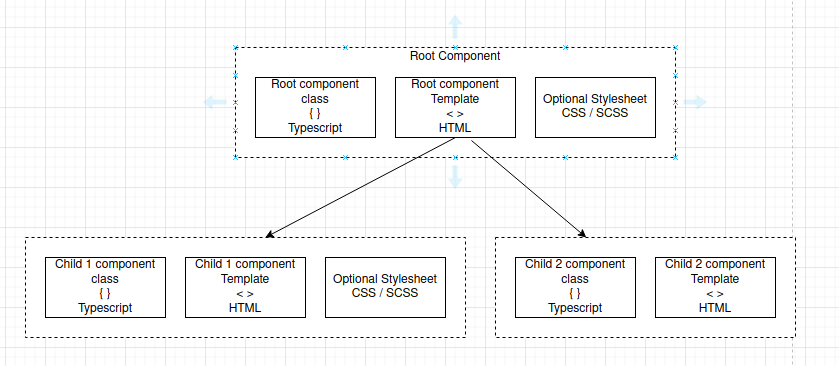
\includegraphics[width=1\linewidth]{images/codeCoverage.png}    

    \caption{ This code coverage table was produced by the testing framework and shows the test coverage for different parts of the program including the typescript classes and Angular components created. 
    }

    % use the notation fig:name to cross reference a figure
    \label{fig:codeCoverage} 
\end{figure}

How good is your solution? How well did you solve the general problem, and what evidence do you have to support that?

\section{Guidance}
\begin{itemize}
    \item
        Ask specific questions that address the general problem.
    \item
        Answer them with precise evidence (graphs, numbers, statistical
        analysis, qualitative analysis).
    \item
        Be fair and be scientific.
    \item
        The key thing is to show that you know how to evaluate your work, not
        that your work is the most amazing product ever.
\end{itemize}

\section{Evidence}





Make sure you present your evidence well. Use appropriate visualisations, reporting techniques and statistical analysis, as appropriate.

If you visualise, follow the basic rules, as illustrated in Figure \ref{fig:boxplot}:
\begin{itemize}
\item Label everything correctly (axis, title, units).
\item Caption thoroughly.
\item Reference in text.
\item \textbf{Include appropriate display of uncertainty (e.g. error bars, Box plot)}
\item Minimize clutter.
\end{itemize}

See the file \texttt{guide\_to\_visualising.pdf} for further information and guidance.

\begin{figure}
    \centering
    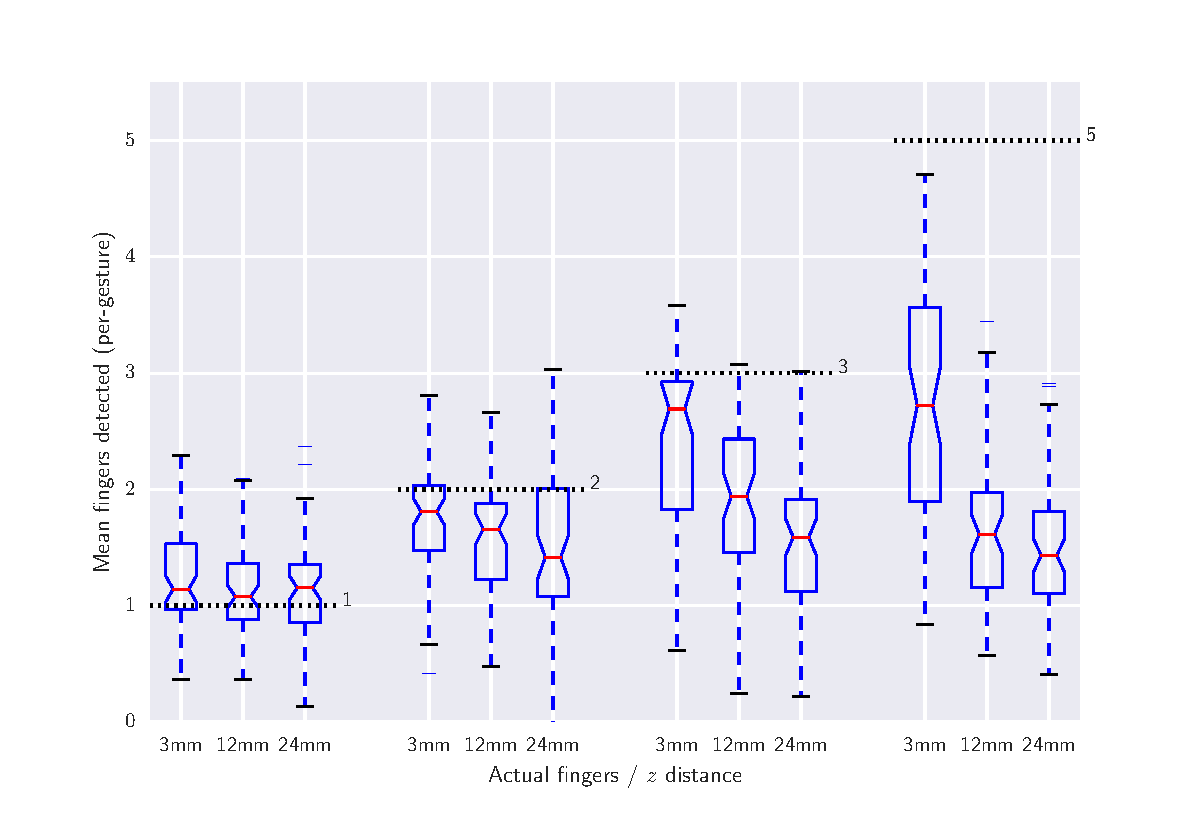
\includegraphics[width=1.0\linewidth]{images/boxplot_finger_distance.pdf}    

    \caption{Average number of fingers detected by the touch sensor at different heights above the surface, averaged over all gestures. Dashed lines indicate
    the true number of fingers present. The Box plots include bootstrapped uncertainty notches for the median. It is clear that the device is biased toward 
    undercounting fingers, particularly at higher $z$ distances.
    }

    % use the notation fig:name to cross reference a figure
    \label{fig:boxplot} 
\end{figure}


%==================================================================================================================================
\chapter{Conclusion}    
Summarise the whole project for a lazy reader who didn't read the rest (e.g. a prize-awarding committee).
\section{Guidance}
\begin{itemize}
    \item
        Summarise briefly and fairly.
    \item
        You should be addressing the general problem you introduced in the
        Introduction.        
    \item
        Include summary of concrete results (``the new compiler ran 2x
        faster'')
    \item
        Indicate what future work could be done, but remember: \textbf{you
        won't get credit for things you haven't done}.
\end{itemize}

%==================================================================================================================================
%
% 
%==================================================================================================================================
%  APPENDICES  

\begin{appendices}

\chapter{Appendices}

Typical inclusions in the appendices are:

\begin{itemize}
\item
  Copies of ethics approvals (required if obtained)
\item
  Copies of questionnaires etc. used to gather data from subjects.
\item
  Extensive tables or figures that are too bulky to fit in the main body of
  the report, particularly ones that are repetitive and summarised in the body.

\item Outline of the source code (e.g. directory structure), or other architecture documentation like class diagrams.

\item User manuals, and any guides to starting/running the software.

\end{itemize}

\textbf{Don't include your source code in the appendices}. It will be
submitted separately.

\end{appendices}

%==================================================================================================================================
%   BIBLIOGRAPHY   

% The bibliography style is abbrvnat
% The bibliography always appears last, after the appendices.

\bibliographystyle{abbrvnat}

\bibliography{l4proj}

\end{document}
